\documentclass[prb,12pt, nofootinbib]{revtex4-2}
%fonts
% Palatino for main text and math
\usepackage[osf,sc]{mathpazo}
% Helvetica for sans serif
% (scaled to match size of Palatino)
\usepackage[scaled=0.90]{helvet}

% Bera Mono for monospaced
% (scaled to match size of Palatino)
\usepackage[scaled=0.85]{beramono}
\usepackage{amsmath, amssymb,physics,amsfonts,amsthm}
\usepackage{enumitem}
\usepackage{cancel}
\usepackage[most]{tcolorbox}
\usepackage{booktabs}
%\usepackage{subcaption}
%\captionsetup[subfigure]{% changed <<<<<<<<<<<<<<<<
%	singlelinecheck = false,
%	justification=raggedright, 
%	margin = {-3ex, 0mm}, % make margin font size dependent
%}
\usepackage{tikz}
\usepackage[caption=false]{subfig}


\usepackage{pgfplots}
\usepackage{wasysym}
\usepackage{listings}
\usepackage{bbm}
\usepackage{hyperref}
\usepackage{enumitem}
\usepackage{transparent}
\usepackage{xcolor}
\usepackage{float}
\usepackage{multirow}
\usepackage[compat=1.1.0]{tikz-feynman}
\usepackage{slashed}
\usepackage[normalem]{ulem}
\theoremstyle{definition}
\newtheorem{Theorem}{Theorem}
\newtheorem{Proposition}{Proposition}
\newtheorem{Lemma}[Theorem]{Lemma}
\newtheorem{Corollary}[Theorem]{Corollary}
\newtheorem{Example}[Theorem]{Example}
\theoremstyle{definition}
\newtheorem{Remark}[Theorem]{Remark}
\theoremstyle{definition}
\newtheorem{Problem}{Problem}
\theoremstyle{definition}
\newtheorem{Definition}[Theorem]{Definition}
\newenvironment{parts}{\begin{enumerate}[label=(\alph*)]}{\end{enumerate}}
\newcommand{\backvec}[1]{\reflectbox{$\vec{\reflectbox{\!$#1$}}$}}

%tikz
\usetikzlibrary{patterns}
\usepackage{tikz-cd}
% definitions of number sets
\newcommand{\N}{\mathbb{N}}
\newcommand{\R}{\mathbb{R}}
\newcommand{\Z}{\mathbb{Z}}
\newcommand{\Q}{\mathbb{Q}}
\newcommand{\C}{\mathbb{C}}
\allowdisplaybreaks

\newcommand{\note}[1]{{\color{red} #1}}
\newtcolorbox{revision}[1][]{empty, breakable, sharp corners, borderline north={1pt}{0pt}{black},
	borderline west={5pt}{0pt}{black},
	#1}

\definecolor{codegreen}{rgb}{0,0.6,0}
\definecolor{codegray}{rgb}{0.5,0.5,0.5}
\definecolor{codepurple}{rgb}{0.58,0,0.82}
\definecolor{backcolour}{rgb}{0.95,0.95,0.92}

\lstdefinestyle{mystyle}{
	backgroundcolor=\color{backcolour},   
	commentstyle=\color{codegreen},
	keywordstyle=\color{magenta},
	numberstyle=\tiny\color{codegray},
	stringstyle=\color{codepurple},
	basicstyle=\ttfamily\footnotesize,
	breakatwhitespace=false,         
	breaklines=true,                 
	captionpos=b,                    
	keepspaces=true,                 
	numbers=left,                    
	numbersep=5pt,                  
	showspaces=false,                
	showstringspaces=false,
	showtabs=false,                  
	tabsize=2,
	literate={_}{{\_}}1
}

\lstset{style=mystyle}

\renewcommand{\note}[1]{{}}
\begin{document}
\title{Tensor Products on Quantum Spin Systems}
	\author{Jun Wei Tan}
	\email{jun-wei.tan@stud-mail.uni-wuerzburg.de}
	\affiliation{Julius-Maximilians-Universit\"{a}t W\"{u}rzburg}
	\date{\today}
	\maketitle
	\begin{tcolorbox}
		In the 1960s Friedrichs met Heisenberg, and used the occasion to express to him the deep gratitude of the community of mathematicians for having created quantum mechanics, which gave birth to the beautiful theory of operators in Hilbert space. Heisenberg allowed that this was so; Friedrichs then added that the mathematicians have, in some measure, returned the favor. Heisenberg looked noncommittal, so Friedrichs pointed out that it was a mathematician, von Neumann, who clarified the difference between a self-adjoint operator and one that is merely symmetric. ``What's the difference,'' said Heisenberg. \cite{lax2014functional}
	\end{tcolorbox}
What is a particle? 

First, \textcolor{red}{To write introduction}

\section{The Quasi-Local Algebra}
In the previous semester, we constructed our observable algebra in a rather ad hoc manner: We declared that we had an algebra $\mathcal{A}(\mathcal{O})$ for each region of spacetime $\mathcal{O}$. Then, we considered only algebras for which the asymptotic abelianness condition held.

However, this ostensibly presents a number of conditions which our algebras have to fulfil. It no longer suffices to write down a model --- we have to then verify that the associated $C^*$ algebra satisfies these conditions. Instead, we will proceed with a more formal construction of the \emph{quasi-local algebra} as defined in \cite{bratteli2012operator}, and show that it satisfies all the conditions we seek.
\begin{Definition}[Quasi-Local Algebra]
	A quasi-local algebra is a $C^*$ algebra $\mathcal{A}$ and a net of $C^*$ algebras $\{\mathcal{A}_\alpha\}_{\alpha\in I}$ such that the net $I$ has an orthogonality relation $\perp$ and that satisfies the fololowing conditions.
	\begin{enumerate}
		\item If $\alpha\ge \beta$, then $\mathcal{A}_\alpha \supseteq \mathcal{A}_\beta$.
		\item $\mathcal{A}=\overline{\cup_\alpha \mathcal{A}_\alpha}$, where the bar denotes norm closure.
		\item The algebras $\mathcal{A}_\alpha$ all share an identity element $\mathbbm{1}$.
		\item There exists an automorphism $\sigma$ with $\sigma^1=\mathbbm{1}$, such that $\sigma(\mathcal{A}_\alpha)=\mathcal{A}_\alpha$ and
			\[
				[\mathcal{A}_\alpha^e, \mathcal{A}_\beta^e]=[\mathcal{A}_\alpha^e, \mathcal{A}_\beta^o] = \{\mathcal{A}_\alpha^o, \mathcal{A}_\beta^o \} = \{0\}
			\] 
			whenever $\alpha\perp \beta$, and $ \mathcal{A}_\alpha^e$ and $\mathcal{A}_\beta^e$ are the even and odd elements with respect to $\sigma$ (meaning those elements with $\sigma(A)=A$ or $\sigma(A) = -A$ respectively)
	\end{enumerate}
\end{Definition}
This definition requires a significant amount of unpacking. First, we have an index set for the algebras. In many applications of physics, this will be include subsets of spacetime, $I\subseteq \mathcal{P}(\R^n)$. They will be ordered by inclusion, and we will declare two subsets orthogonal if they are disjoint.

The last condition also requires some explanation. Essentially, if we have two bosonic operators that are spacetime separated, we expect that they commute; while if we have fermionic operators, we expect that they anticommute. Thus, even asymptotically, we must distinguish between these two types. The automorphism takes care of this; in some sense, the even elements represent the bosonic operators and the even ones the fermionic operators.

Having constructed appropriate algebras for each region of spacetime, we then find the quasi-local algebra by taking the norm closure of their union.

In this talk, we will mostly work with \uline{spin systems}. In a spin system, we have as our spacetime $\Z^n$ instead of $\R^n$. Physically, these could represent atoms, and the electrons can only hop between these atoms. We call this a tight binding model. The $C^*$ algebra for a single spin is also given by the $2\times 2$ matrices.
\begin{figure}
	\begin{center}
		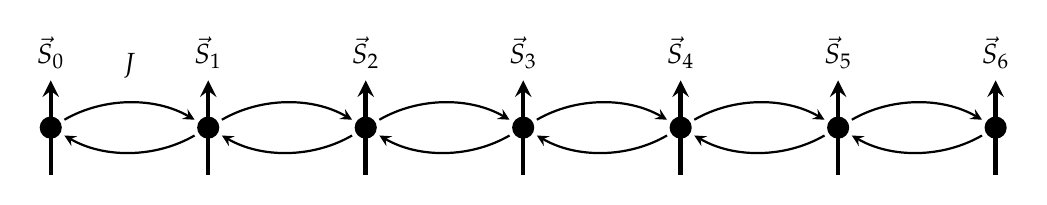
\begin{tikzpicture}[scale=2]
			\foreach \x in {0,1, ..., 6}
			{
				\fill (\x,0) circle (2pt);
				\draw[ultra thick,-stealth] (\x,-0.3) -- (\x, 0.3) node[anchor=south] {$\vec{S}_{\x}$};
			}
			
			\foreach \x in {0,1, ..., 5}{
				\draw[thick, -stealth, shorten <= 0.2cm, shorten >= 0.2cm] (\x, 0) to[bend left=30] ({\x+1},0);
				\draw[thick, -stealth, shorten <= 0.2cm, shorten >= 0.2cm] ({\x+1}, 0) to[bend left=30] ({\x},0);
			}
			
			\draw (0.5,0.25) node[anchor=south] {$J$};
		\end{tikzpicture}
	\end{center}
	\caption{The Heisenberg model in 1 dimension is pictured. At each lattice site, there is a single spin; an energy penalty $J$ is applied for every two spins that are pointing in the same direction.}
	\label{fig:heisenberg}
\end{figure}
\begin{Example}
	The Heisenberg model consists of a lattice of spins as pictured in Fig.~\ref{fig:heisenberg}. Each spin interacts with each other through a Hamiltonian
	\[
		H = J\sum_{\langle ij\rangle} \vec{S}_i \cdot \vec{S}_j
	\] 
	where $\langle ij\rangle$ means that they are only summed over if $i$ and $j$ are neighbours. It can be shown that the ground state of this model is ferromagnetic for $J<0$ and antiferromagnetic for $J>0$.
\end{Example}

\section{Dynamics of Quantum Systems}
Having the algebra, we must next be able to define the dynamics of a quantum system. While it is possible to define the dynamics using a Hamiltonian in the GNS representation, this defeats the purpose of the algebraic approach to quantum mechanics. Thus, we seek with a purely $C^*$ algebraic way to generate dynamics. Let us begin with the goal:

\begin{Definition}
	A time evolution on a $C^*$ algebra $\mathcal{A}$ is an function $\alpha: \mathcal{A}\times \R\to \mathcal{A}$, that we denote as $\alpha_t$, such that each $\alpha_t$ is an automorphism.
\end{Definition}

In the case where $\mathcal{A}$ has the form $\mathcal{B}(\mathcal{H})$, we can prove that the automorphisms are \emph{inner}, meaning that they can be represented as a unitary time evolution
\[
\alpha_t(A) = U(t)AU(t)^*
.\] 
Then, using Stone's theorem, we can represent $U$ as an exponential $\exp(itH)$, yielding our Hamiltonian. However, this requires a Hilbert space, and hence is not desirable. Instead, the generator of dynamics on a $C^*$ algebra is known as a \emph{derivation}:
\begin{Definition}
	A derivation $\delta$ of a $C^*$ algebra is a linear map defined on a *-subalgebra $D(\delta)$, $\delta:D(\delta)\to \mathcal{A}$ such that
	\begin{enumerate}
		\item $\delta(A^*)=\delta(A)^*$ for $A\in D(\delta)$ 
		\item $\delta(AB)=\delta(A)B+A\delta(B)$ for $A,~B\in D(\delta)$.
	\end{enumerate}
\end{Definition}
Essentially, the product rule suffices to define a derivative. This is reminiscent of differential geometry, where the tangent space is defined using derivations in a very similar manner. 

This construction satisfies many of the properties we might expect. We will state a few examples without proof.
\begin{Example}
	Consider a $C^*$ algebra $\mathcal{A}$ with a strongly continuous 1 parameter group of automorphisms $\alpha_t$, meaning that $t\mapsto \alpha_t(A)$ is strongly continuous for each $A$. Then
	\[
	\delta(A) = \lim_{t \to 0}\left( \frac{\alpha_t(A) - A}{t} \right)  
\]
is a derivation, defined on the points where the limit exists.
\end{Example}
In a unitary time evolution on a Hilbert space, the corresponding derivation is given by the commutator as we might expect.
\begin{Example}
	Consider $\mathcal{A}=\mathcal{B}(\mathcal{H})$ and let $\alpha_t$ be a 1 parameter group of automorphisms given by conjugation:
	\[
		\alpha_t(A) = e^{itH}Ae^{-itH}
	\]
	for self-adjoint $H$. Then the corresponding derivation is given by
	\[
		\delta(A) = i[H,A]
	.\] 
\end{Example}
Now that we have defined derivations, we move forward to define interactions. 
\begin{Definition}
	Consider a quantum spin system defined on a set of sites $\Gamma$. An interaction $\Phi$ is a mapping $\Phi: \mathcal{P}(\Gamma)\to \mathcal{A}$ such that $\Phi(\Lambda)\in \mathcal{A}(\Lambda)$ and $\Phi(\Lambda)$ is self adjoint.
\end{Definition}
\begin{Example}
	In the Heisenberg model, we have
	\[
	\Phi(\{x,y\}) = \begin{cases}
		J & \langle xy\rangle\\
		0 & \text{otherwise.}
	\end{cases}
	\] 
\end{Example}
We recall again that we are working with \emph{spin systems}. This will become important here. In particular, it is important that the algebra on each site is finite. That means, if $\Lambda$ is bounded, then $\Phi(\Lambda)$ is finite dimensional. Thus, for each $\Lambda$, we can construct a \emph{bounded} Hamiltonian via
\[
	H(\Lambda) = \sum_{X\subseteq \Lambda}\Phi(X)
.\] 
In addit.ion, the interactions will also often be \emph{finite range}, meaning that $\Phi(X)=0$ for sets larger than a certain diameter, say $|X| > N_\Phi$. If the interaction is finite range, then the sum of the local Hamiltonians induce a derivation, because
\[
	\delta^n(A) = i \lim_{\Lambda \to \infty}[H_\Lambda, A]
\]
only has finitely many terms where $H_\Lambda$ intersects $A$.\note{ Probably comment something here about how this limit is in the sense of convergence of a net in the sense of the quasi-local algebra.}

We will call the $C^*$ algebra the local algebra $\mathcal{A}_\text{loc}$ and the corresponding Hamiltonians the local Hamiltonians. Because of this, we can then show the time evolution for local systems:
\begin{figure}
	\begin{center}

\subfloat[][ ]{%
  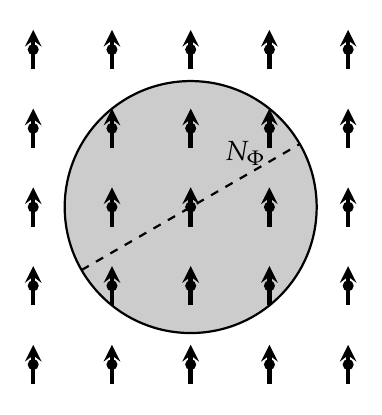
\begin{tikzpicture}
	  \foreach \x in {0, ..., 4}
	  \foreach \y in {0, ..., 4}
	  {
	  \draw[ultra thick, -stealth] ({\x}, {\y-0.25}) -- ++(0,0.5);
	  \fill (\x, \y) circle (2pt);
	  }
	  \filldraw[thick,fill opacity=0.2] (2,2) circle (1.6);
	  \draw[thick, dashed] ({2-1.6*cos(30)}, {2-1.6*sin(30)}) -- ({2+1.6*cos(30)}, {2+1.6*sin(30)});
	  \draw ({2+0.8*cos(30)}, {2+0.8*sin(30)}) node[anchor=south] {$N_\Phi$};
  \end{tikzpicture}
}
\hfill
\subfloat[][ ]{%
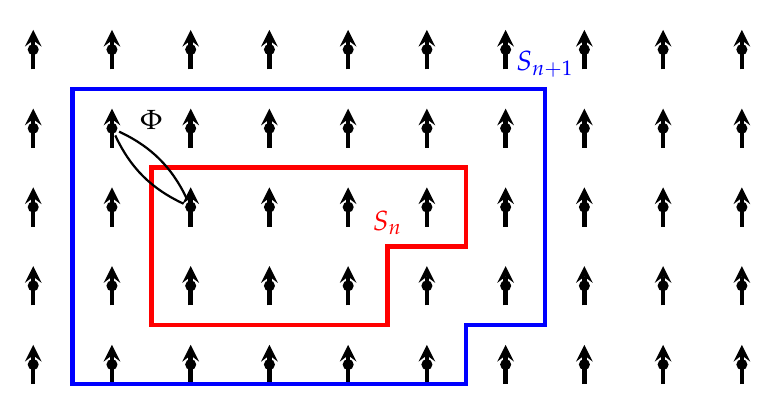
\begin{tikzpicture}
	\foreach \x in {0, ..., 9}
	\foreach \y in {0, ..., 4}
	{
	\fill (\x, \y) circle (2pt);
	\draw[ultra thick, -stealth] (\x, {\y-0.25}) -- ++(0,0.5);
	}
	\draw[ultra thick, red] (1.5,0.5) -- ++(3,0) -- ++(0,1) node[anchor=south, red] {$S_n$} -- ++(1,0) -- ++(0,1) -- ++(-4,0) -- cycle;
	\draw[ultra thick, blue] (0.5,-0.25) -- ++(5,0) -- ++(0,0.75) -- ++(1,0) -- ++(0,3) node[anchor=south, blue] {$S_{n+1}$}-- ++(-6,0) -- cycle;
	\draw[thick, shorten <= 0.1cm, shorten >= 0.1cm] (2,2) to[bend left=20] (1,3);
	\draw[thick, shorten <= 0.1cm, shorten >= 0.1cm] (2,2) to[bend right=20] (1,3);
	\draw (1.5,3.1) node {$\Phi$};
\end{tikzpicture}
}
	\end{center}
	\caption{Structure of local interactions. \textbf{(a)} If the interaction is local, there is a number $N_\Phi$ such that $\Phi(X)$ is only nonzero for sets smaller than $N_\Phi$ (as pictured). \textbf{(b)} Given an observable with support in the set $S_n$, application of the commutator allows for interactions within slightly wider sets, as shown in $S_{n+1}$.}
	\label{fig:interactions}
\end{figure}
\begin{Theorem}
	Let $\Phi$ be a finite range interaction and $\delta$ the corresponding derivation. Then the local algebra $\mathcal{A}_\text{loc}$ is analytic, meaning that $\exp(t\delta)(A)$ exists for all $A\in \mathcal{A}_\text{loc}$ and sufficiently small $t$.
\end{Theorem}
\begin{proof}
	Essentially we want to bound $\|\delta^n(A)\|$. In expectation that the locality of $A$ will be important, we define a \emph{finite} set $\Lambda$ such that $A\in \mathcal{A}(\Lambda)$. If there existed a Hamiltonian $H$ corresponding to the interaction, we would have 
	\[
		\delta^n(A) = i^n [H, [\dots, [H, A]] 
	.\] 
	However, there is no Hamiltonian for the entire interaction. However, the finite range nature of the interaction now comes into play. For example, in the first commutator, we would have
	\[
		\delta(A) = i \sum_{X_1|X_1\cap \Lambda \neq \emptyset } [\Phi(X_1), A]
	.\] 
	Here, the locality of the algebra means that the commutator is only nonvanishing for $X_1$ that intersect $\Lambda$, and thus we only need to consider these sets. Because $\Lambda$ is finite, the number of possible $X_1$ is also finite, and thus the sum must be finite. In the general case, we define $S_1=\Lambda$ and $S_k = S_{k-1}\cup X_{k-1}$ for $k>1$ (see Fig.~\ref{fig:interactions}). Then, 
	\[
		\delta^n(A)=i^n \sum_{X_1\cap S_1 \neq \emptyset }\dots \sum_{X_n \cap S_n \neq \emptyset} [\Phi(X_n), [\dots, [\Phi(X_1), A]]]
.\] 
The missing ingredient is a bound on the number of possible subsets $X_n$. Since the interaction is finite range, there is a constant $N_\Phi$ such that it suffices to consider $X_n$ with $|X_n| \le N_\Phi$. Thus, we have
\[
\|\delta^n(A)\|\le 2^n \|A\|\prod_{k=1}^{n} ((k-1)(N_\Phi-1)+|\Lambda|)\|\Phi\|^n 
.\] 
By a simple computation, it follows that
\[
	\|\delta^n(A)\|\le \|A\|n! e^{\lambda(|\Lambda|+1-N_\Phi)}\left( \frac{2\|\Phi\|e^{\lambda(N_\Phi-1)}}{\lambda} \right)^n
.\] 
Thus, the exponential exists for sufficiently small $t$.
\end{proof}
Now that we have constructed the exponential for local observables, we must extend it to the entire quasi-local algebra in the following theorem:
\begin{Theorem}
	There exists a one parameter group of automorphisms $\alpha_t$ on the quasi-local algebra $\mathcal{A}$.
\end{Theorem}
\begin{proof}
	We will extend the group as follows. \note{Write this part in bullet points }First, we will begin with an interaction on a finite region. This will allow us to show isometry, which will then provide an extension to the quasi local algebra using well known results. Finally, we will extend the domain of $t$ from a neighbourhood of the origin to the entire real line.

	We begin by defining $\delta_{\Lambda}(A)  = i[H_{\Lambda}, A]$ for a finite subset $\Lambda$ of the sites. We also begin with a local operator $A\in \mathcal{A}(X)$. For each $\Lambda\supseteq X$, the derivations $\delta^n(A)$ and $\delta_{\Lambda}^n(A)$ will agree for $n\le N(\Lambda)$, where $N(\Lambda)$ is some function depending on $\Lambda$\note{~Probably draw here a picture about how the correlations spread}. Thus, we have
	\[
		\|\alpha_t^\Lambda(A) - \alpha_t(A)\|= \left\|\sum_{n=N(\Lambda)}^\infty \left( \frac{t^n\delta_{\Lambda}^n(A)}{n!} - \frac{t^n \delta^n(A)}{n!} \right) \right\|
	.\] 
	Note that $N(\Lambda)\xrightarrow{\Lambda\to\infty}\infty$. \textcolor{red}{Complete proof later}
\end{proof}
Now that dynamics have been defined, the final ingredient we need is to define ground states. 
\section{Ground States}
Ground states are states of minimal energy. Since this does not affect the dynamics, we can always shift the zero of energy such that the ground state has zero energy\note{~Probably write down the derivation and show that the thing commutes}. Thus, ground states do not evolve in time\note{~Write down the $\exp(-iHt)$ expression here}. This leads us to our formal definition
\begin{Definition}
	Let $\alpha_t$ be a 1 parameter group of automorphisms on a $C^*$ algebra $\mathcal{A}$. Then a ground state $\omega$ is a state such that $\omega\circ \alpha_t=\omega$ for all $t$ and if $H_\omega\ge 0$ in the corresponding GNS representation\note{~The important point here is that even though the derivation $\delta$ exists on $\Lambda\to\infty$, $H$ does not, because it is unbounded; hence, we can only verify positivity in the GNS representation}.
\end{Definition}
However, this definition is clearly unwieldy, not least because we need to explicitly construct the Hamiltonian in the GNS representation. Instead, we seek another characterisation of ground states, which we will state without proof
\begin{Theorem}
	\label{thm:groundstate}
	Let $\omega$ be a state on $\mathcal{A}$ and $\alpha_t$ a strongly continuous 1 parameter group of automorphisms. Then the following are equivalent
	\begin{enumerate}
		\item $\omega$ is a ground state.
		\item $-i\omega(A^*\delta(A))\ge 0$ for all $A\in D(\delta)$.
	\end{enumerate}
\end{Theorem}
It is then finally time to discuss one of the system that characterised research in the 2000s.
\section{The Toric Code}
\begin{figure}
\begin{center}
	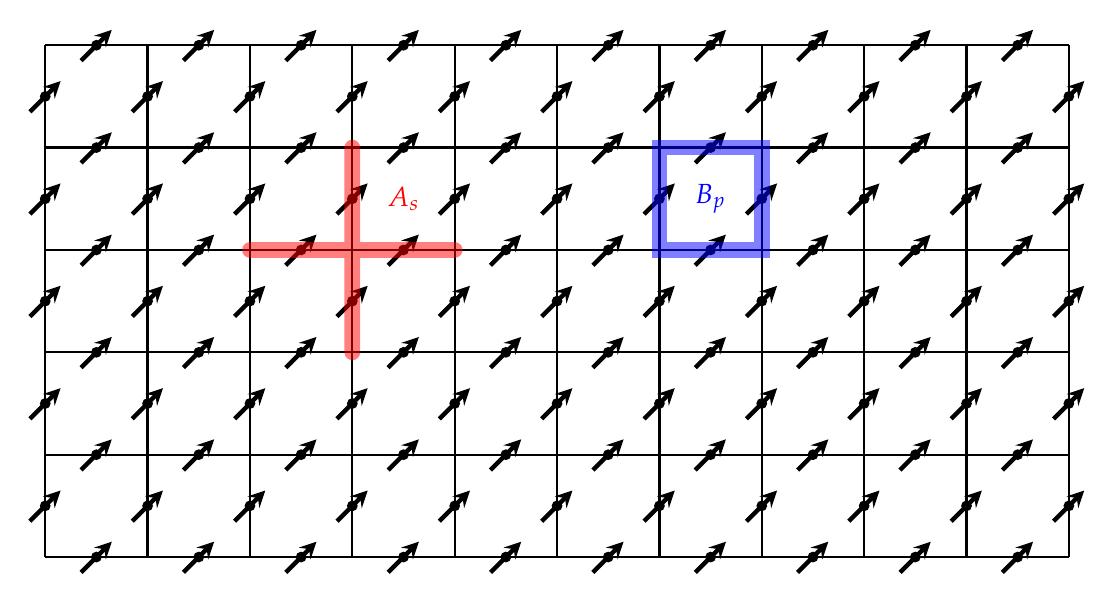
\begin{tikzpicture}[scale=1.3]
	%	\foreach \x in {0,..., 10}
	%	{
	%		\foreach \y in {0, ..., 5}
		%\fill (\x, \y) circle (2pt);
		%\foreach \y in {0, ..., 4}
		%\draw[thick] (\x, \y) -- ++(0,1);
		%}

		%\foreach \x in {0, ..., 9}
		%\foreach \y in {0, ..., 5}
		%\draw[thick] (\x, \y) -- ++(1,0);
		
		\draw[step=1.0, black, thick] (0,0) grid (10,5);

		\foreach \y in {0.5, 1.5, ..., 4.5}
		\foreach \x in {0, ..., 10}
		{
			\fill (\x, \y) circle (1.5pt);
		\draw[ultra thick, -stealth] ({\x-0.15}, {\y-0.15}) -- ++(0.3,0.3);
}
		\foreach \x in {0.5, ..., 9.5}
		\foreach \y in {0, ..., 5}
		{
			\fill (\x, \y) circle (1.5pt);
		\draw[ultra thick, -stealth] ({\x-0.15}, {\y-0.15}) -- ++(0.3,0.3);
}
		\begin{scope}[opacity=0.5, transparency group]
		\draw[line width=2mm, red, line cap = round] (2,3) -- (4,3);
		\draw[line width=2mm, red, line cap = round] (3,2) -- (3,4);
	\end{scope}

		\draw[line width=2mm, blue, line cap = round, opacity=0.5] (6,4) -- (6,3) -- (7,3) -- (7,4) -- cycle;
		\draw (3.5,3.5) node[red] {$A_s$};
		\draw (6.5,3.5) node[blue] {$B_p$};
	\end{tikzpicture}
	\caption{The toric code consists of a square lattice. A spin degree of freedom lies on each \emph{bond}. The support of the operators $A_s$ and $B_p$ are also drawn.}
	\label{fig:toriccode}
\end{center}
\end{figure}
The Toric code, first proposed by Kitaev \cite{kitaev2003fault} in 1997, remains a paradigmatic model of topological physics. It is defined on a square lattice, with a spin degree of freedom on each \emph{edge}. We then define two operators, one defined on a ``star'' and one on a plaquette (see Fig. \ref{fig:toriccode}):
\[
	A_s = \bigotimes_{j\in s}\sigma_j^x,\qquad B_p = \bigotimes_{j\in p}\sigma_j^z
.\] 
We note that $A_s^2 = B_p^2 = \mathbbm{1}$, and that $[A_s, B_p]=0$ for all stars $s$ and plaquettes $p$. In particular, the eigenvalues of $A_s$ and $B_p$ are $\pm 1$. Now we seek a ground state. Let us begin by showing that $A_s$ and $B_p$ are \emph{stabilisers}.
\begin{Lemma}
	Let $\mathcal{A}$ be a unital $C^*$ algebra,  $\omega$ a state on $\mathcal{A}$. Define $X\in \mathcal{A}$ such that $X=X^*$, $\omega(X)=1$ and $I-X$ is positive. Then for all $Y\in \mathcal{A}$ we have $\omega(XY)=\omega(YX)=\omega(Y)$.
\end{Lemma}
\begin{proof}
	Because $\mathbbm{1}-X$ is positive, we can take the square root $\mathbbm{1}-X$. Then, we have
	\begin{align*}
		|\omega( (\mathbbm{1}-X)Y)|^2 &= |\omega(\sqrt{\mathbbm{1}-X}\sqrt{\mathbbm{1}-X}|^2  \\ 
		&\le \omega(\mathbbm{1}-X)\omega(Y^* (\mathbbm{1}-X)Y)=0 
	\end{align*}
	\note{Write down the fact that $\omega( (\mathbbm{1}-X)Y)=0$ }where we used the Cauchy-Schwarz inequality before finding that $\omega(\mathbbm{1}-X)=0$. Similarly, we can show that $\omega(Y(\mathbbm{1}-X))=0$. Thus, by the linearity of states, we find that $\omega(XY)=\omega(YX)=\omega(Y)$. 
\end{proof}
Now, we show the stabilisor property of $A_s$ and $B_p$:
\begin{Theorem}
Let $\omega$ be a state on $\mathcal{A}$ such that $\omega(A_s)=\omega(B_p)=1$ for all $s$ and $p$. Then $\omega$ is a ground state.
\end{Theorem}
\begin{proof}
	Again, we consider a local $A\in \mathcal{A}(\Lambda)$. Then, the derivation is given by
	\[
	\delta(A) = -i \sum_{s\cap \Lambda \neq \emptyset} [A_s, A] - i \sum_{p\cap \Lambda\neq\emptyset} [B_p, A]
	\] 
	where we have summed over the stars $s$ and the plaquettes $p$ intersecting $\Lambda$. We seek to use Theorem \ref{thm:groundstate} to prove that $\omega$ is a ground state. Thus, we expand\note{ Note that $\mathbbm{1}-A_s$ is positive because $A_s$ is a projector}
	\[
	-i\omega(A^*\delta(A))=\sum_{s\cap\Lambda\neq\emptyset} \omega(A^*A A_s)-\omega(A^*A_sA)+\sum_{p\cap\Lambda\neq\emptyset}\omega(A^*AB_p)-\omega(A^*B_pA)
	.\] 
	However, using the previous lemma and the condition that $\omega(A_s)=1$, we can write $\omega(A^*A A_s)=\omega(A^* A)$ and thus
	\[
	\omega(A^*A)-\omega(A^* A_s A)=\omega(A^* (\mathbbm{1}-A_s)A)\ge 0
	.\] 
	Thus, we find that the expression is positive, and $\omega$ is then a ground state.
\end{proof}
What do such states look like? Since $A_s$ or $B_p$ are the product of four spin operators, if we flip an even number of spins, $A_s$ or $B_p$ will not change in value. Thus, if we look at only the star or the plaquette operators, flipping spins in a loop will not affect their value. Joining the flipped spins together, we can construct ``ground states'' for the star and plaquette operators respectively (see Fig. \ref{fig:loopgas}).

\begin{figure}
	\begin{center}
		
		\subfloat[][ ]{%
			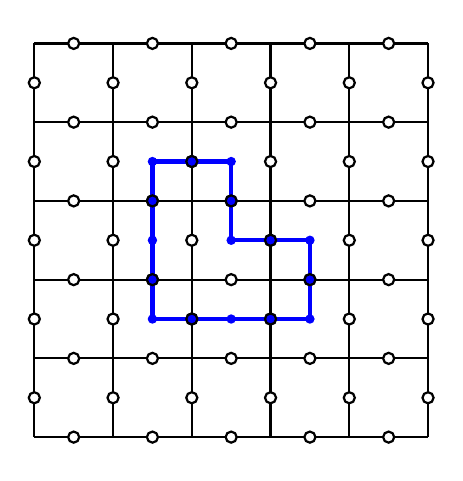
\begin{tikzpicture}
				
				\fill[opacity=0] (0,5) rectangle (0.2,5.2);
				\fill[opacity=0] (0,0) rectangle (0.2,-0.2);
				\draw[thick] (0,0) grid (5,5);
				
				\foreach \x in {0, ..., 5}
				\foreach \y in {0.5, ..., 4.5}
				\filldraw[fill=white,draw=black,thick] (\x, \y) circle (2pt);
				
				\foreach \x in {0.5, ..., 4.5}
				\foreach \y in {0, ..., 5}
				\filldraw[fill=white,draw=black,thick] (\x, \y) circle (2pt);
				
				\draw[ultra thick, blue] (1.5, 1.5) -- ++(2,0) -- ++(0,1) -- ++(-1,0) -- ++(0,1) -- ++(-1,0) -- cycle;
				\filldraw[fill=blue,draw=black,thick] (1.5, 2) circle (2pt);
				\filldraw[fill=blue,draw=black,thick] (1.5, 3) circle (2pt);
				\filldraw[fill=blue,draw=black,thick] (3.5, 2) circle (2pt);
				\filldraw[fill=blue,draw=black,thick] (2.5, 3) circle (2pt);
				\filldraw[fill=blue,draw=black,thick] (2, 1.5) circle (2pt);
				\filldraw[fill=blue,draw=black,thick] (3, 1.5) circle (2pt);
				\filldraw[fill=blue,draw=black,thick] (2, 3.5) circle (2pt);
				\filldraw[fill=blue,draw=black,thick] (3, 2.5) circle (2pt);
				
		%		\foreach \x in {3.5, ..., 4.5}
		%		\foreach \y in {3.5, ..., 4.5}
		%		{
			%		\fill (\x, \y) circle (1.7pt);
				%\draw[thick, -stealth] (\x, {\y -0.2}) -- ++(0,0.4);
			%}
			
			%\foreach \x in {0.5, ..., 4.5}
			%{
			%	\fill (\x, 0.5) circle (1.7pt);
				%\draw[thick, -stealth] (\x, {0.5 -0.2}) -- ++(0,0.4);
			%}
			
			%\foreach \y in {1.5, ..., 4.5}
			%{
			%					\fill (0.5, \y) circle (1.7pt);
			%\draw[thick, -stealth] (0.5, {\y -0.2}) -- ++(0,0.4);
			%}
			
			%\foreach \x in {1.5, 2.5}{
			%\fill (\x, 4.5) circle (1.7pt);
			%\draw[thick, -stealth] (\x, {4.5-0.2}) -- ++(0,0.4);
		%}
		
		%\foreach \y in {1.5, 2.5}{
	%					\fill (4.5, \y) circle (1.7pt);
			%\draw[thick, -stealth] (4.5, {\y -0.2}) -- ++(0,0.4);
		%}
			
						\foreach \y in {1.5, ..., 3.5}
						\foreach \x in {1.5, 2.5}
			{
				\fill[blue] (\x, \y) circle (1.7pt);
				%\draw[thick, -stealth, blue] (\x, {\y +0.2}) -- ++(0,-0.4);
			}
			
									\foreach \y in {1.5, 2.5}
			{
				\fill[blue] (3.5, \y) circle (1.7pt);
				%\draw[thick, -stealth, blue] (3.5, {\y +0.2}) -- ++(0,-0.4);
			}
			
			\end{tikzpicture}
		}
		\hspace{1cm}
		\subfloat[][ ]{%
			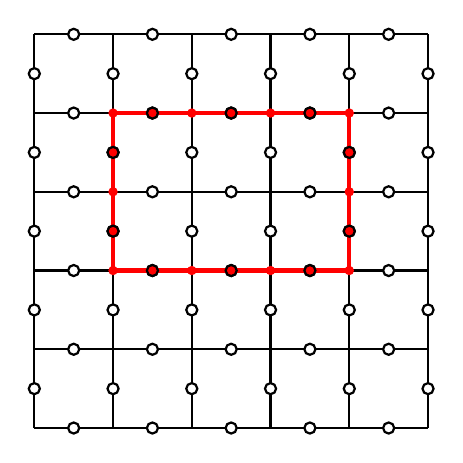
\begin{tikzpicture}
				\draw[thick] (0,0) grid (5,5);
								\foreach \x in {0, ..., 5}
				\foreach \y in {0.5, ..., 4.5}
				\filldraw[fill=white,draw=black,thick] (\x, \y) circle (2pt);
				
				\foreach \x in {0.5, ..., 4.5}
				\foreach \y in {0, ..., 5}
				\filldraw[fill=white,draw=black,thick] (\x, \y) circle (2pt);
				
				\draw[ultra thick, red] (1,2) -- ++(3,0) -- ++(0,2) -- ++(-3,0) -- cycle;
				
				\foreach \x in {1.5, ..., 3.5}
				\foreach \y in {2, 4}
				\filldraw[fill=red,draw=black,thick] (\x, \y) circle (2pt);
				
				\foreach \x in {1, 4}
				\foreach \y in {2.5, 3.5}
				\filldraw[fill=red,draw=black,thick] (\x, \y) circle (2pt);
				
				%\foreach \x in {0, ..., 5}
				%\foreach \y in {0,1, 5}
				%{
				%\fill (\x, \y) circle (1.7pt);
				%\draw[thick, -stealth] (\x, {\y-0.2}) -- ++(0,0.4);
				%}
				
				%\foreach \x in {0, 5}
				%\foreach \y in {2, ..., 4}
				%{
				%				\fill (\x, \y) circle (1.7pt);
			%	\draw[thick, -stealth] (\x, {\y-0.2}) -- ++(0,0.4);
				%}
				
				\foreach \x in {1, ..., 4}
				\foreach \y in {2, 4}
				{								\fill[red] (\x, \y) circle (1.7pt);
				%	\draw[thick, -stealth, red] (\x, {\y+0.2}) -- ++(0,-0.4);
				}
				
				\foreach \x in {1,4}
				\fill [red] (\x, 3) circle (1.7pt);
			\end{tikzpicture}
		}
	\end{center}
	\caption{Loop gas of the toric code corresponds to an Ising model. \textbf{(a)} The spins corresponding to the plaquettes, when flipped, create a loop defined on the \emph{dual} lattice to the square lattice. \textbf{(b)} The spins corresponding to the stars create a loop within the original square lattice when flipped.}
	\label{fig:loopgas}
\end{figure}
What about the ground state of the total Hamiltonian? Consider a loop formed on the lattice such as in Fig. \ref{fig:loopgas}(b). Notice that applying $B_p$ to a square within the loop does not change the loop structure\note{ Draw it out}. Thus, we conclude that the ground state must be invariant under the action of $B_p$. There is only one way for this to be true --- the ground state must be an invariant superposition of \emph{all} possible loops. Mathematically, the existence of this state is surprisingly easy to prove. We begin by defining an algebra that essentially captures all the relevant properties of the system. 

\begin{Definition}
	The classical algebra of the toric code is defined by
	\[
	\mathcal{A}_\text{cl} = \mathcal{A}(\{A_s\}, \{B_p\} ) 
	\] 
	i.e. it is the algebra generated by the operators $A_s$ and $B_p$.
\end{Definition}
As we now know, an abelian $C^*$ algebra admits a realisation as a set of continuous functions via the Gel'fand transformation~\cite{takesaki1979theory}. Since the eigenvalues of $A_s$ and $B_p$ are $\pm 1$, a character must send each element to $\pm 1$. Thus, a homomorphism $\chi: \mathcal{A}_\text{cl}\to \C$ can be uniquely defined by giving $\chi(A_s)$ and $\chi(B_p)$ a value in $\{-1,1\} $ for each $s$ and $p$. This can be interpreted as mapping each star and plaquette into a spin. Thus, the spins and plaquettes correspond to Ising models. Then, we choose the state with all spins pointing upwards. By the Hahn-Banach theorem, this state extends to a state on $\mathcal{A}$. It can be shown that this is the only translationally invariant ground state.

\begin{figure}
		\subfloat[][ ]{%
	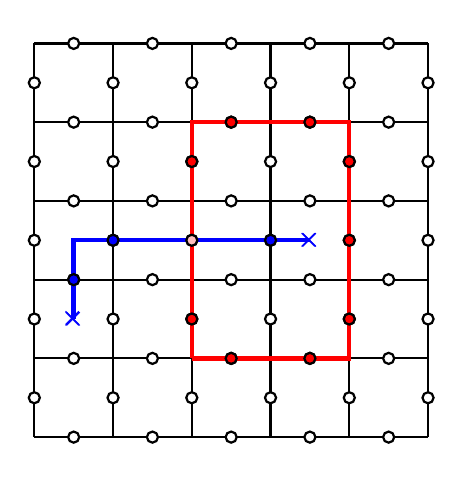
\begin{tikzpicture}
		
		\fill[opacity=0] (0,5) rectangle (0.2,5.2);
		\fill[opacity=0] (0,0) rectangle (0.2,-0.2);
		\draw[thick] (0,0) grid (5,5);
		
		\foreach \x in {0, ..., 5}
		\foreach \y in {0.5, ..., 4.5}
		\filldraw[fill=white,draw=black,thick] (\x, \y) circle (2pt);
		
		\foreach \x in {0.5, ..., 4.5}
		\foreach \y in {0, ..., 5}
		\filldraw[fill=white,draw=black,thick] (\x, \y) circle (2pt);
		
		
		\draw[ultra thick, blue] (0.5,1.5) node[align=center] {$\pmb{\times}$} -- (0.5,2.5) -- (3.5, 2.5) node[align=center] {$\pmb{\times}$};
		\foreach \x in {1,3}
		\filldraw[fill=blue,draw=black, thick] (\x, 2.5) circle (2pt); 
		\filldraw[fill=blue,draw=black, thick] (0.5, 2) circle (2pt);
		\draw[ultra thick, red] (2,1) -- ++(2,0) -- ++(0,3) -- ++(-2,0) -- ++(0,-3); 
		\foreach \x in {2.5, 3.5}
		\foreach \y in {1, 4}
		\filldraw[fill=red,draw=black,thick] (\x, \y) circle (2pt);
		
		\foreach \x in {2, 4}
		\foreach \y in {1.5, 3.5}
		\filldraw[fill=red,draw=black,thick] (\x, \y) circle (2pt);
		
		\filldraw[fill=red,draw=black,thick] (4, 2.5) circle (2pt);
		\filldraw[fill=pink,draw=black,thick] (2, 2.5) circle (2pt);
	\end{tikzpicture}
}
\hspace{1cm}
\subfloat[][ ]{%
	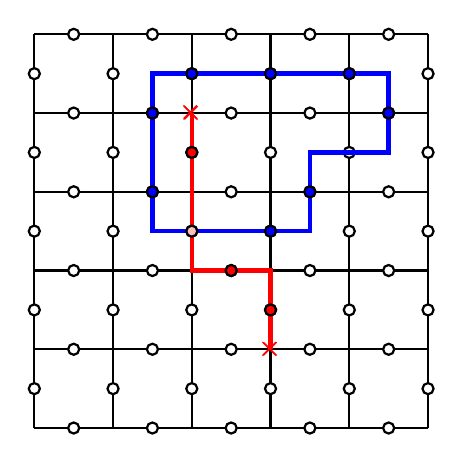
\begin{tikzpicture}
		\draw[thick] (0,0) grid (5,5);
		\foreach \x in {0, ..., 5}
		\foreach \y in {0.5, ..., 4.5}
		\filldraw[fill=white,draw=black,thick] (\x, \y) circle (2pt);
		
		\foreach \x in {0.5, ..., 4.5}
		\foreach \y in {0, ..., 5}
		\filldraw[fill=white,draw=black,thick] (\x, \y) circle (2pt);
		
		\draw[ultra thick, red] (2, 4) node[align=center] {$\pmb{\times}$} -- ++(0,-2) -- ++(1,0) -- ++(0,-1) node[align=center] {$\pmb{\times}$};
		
		\draw[ultra thick, blue] (1.5,2.5) -- ++(2,0) -- ++(0,1) -- ++(1,0) -- ++(0,1) -- ++(-3,0) -- cycle;
		
		\foreach \x in {2, ..., 4}
		\filldraw[fill=blue,draw=black, thick] (\x, 4.5) circle (2pt); 
		\filldraw[fill=blue,draw=black, thick] (1.5, 4) circle (2pt); 
		\filldraw[fill=blue,draw=black, thick] (1.5, 3) circle (2pt); 
		\filldraw[fill=blue,draw=black, thick] (4.5, 4) circle (2pt); 
		\filldraw[fill=blue,draw=black, thick] (3.5, 3) circle (2pt); 
		\filldraw[fill=blue,draw=black, thick] (3, 2.5) circle (2pt); 
		
		\filldraw[fill=red,draw=black, thick] (3, 1.5) circle (2pt);
		\filldraw[fill=red,draw=black, thick] (2.5, 2) circle (2pt);  
		\filldraw[fill=red,draw=black, thick] (2, 3.5) circle (2pt);
		
		\filldraw[fill=pink,draw=black, thick] (2, 2.5) circle (2pt);    
	\end{tikzpicture}
}
	\caption{Detection of defects using Wilson loops. \textbf{(a)} An electric defect is detected using a Wilson loop of star operators. \textbf{(b)} A magnetic defect is detected using a Wilson loop of plaquette operators.}
	\label{fig:wilsonloop}
\end{figure}

\section{Excitations of the Toric Code}
\subsection{Construction of the Excitations}
What would a state that is not a ground state look like? Suppose that one of the $A_s$ has eigenvalue $-1$. Clearly, they cannot come alone; they must come in (at least) pairs. Thus, an excitation could consist of a (noncyclic) path of flipped spins. These are called electric, or e type defects. Similarly, we can create magnetic type defects from broken chains on the reciprocal lattice.

Clearly, this is not a particle type excitation, because it is equivalent to the ground state: By moving the ends of the path, we could get them to touch, thus annihilating each other. 

Where do we look for a particle type excitation? We know that there is essentially only one irreducible representation of a finite dimensional $C^*$ algebra. Therefore, to find particle type excitations, we must look at infinite dimensional $C^*$ algebras, i.e. the thermodynamic limit.

The problem previously was that we could force the two sides to annihilate each other. What if we sent one to infinity?

\begin{Definition}
	Let $\xi$ be a finite nonintersecting path on the lattice. Then we define the path operator $F_\xi = \otimes_{j\in \xi}\sigma_j^z$. 
\end{Definition}

Now, we are in a position to define our particles

\begin{Definition}
	Let $\xi_n$ be a family of paths with the same starting point, but such that the ending point goes to infinity as $n\to\infty$. Define
	\[\rho(A) = \lim_{n\to\infty} F_{\xi_n}AF_{\xi_n}^*.\]
\end{Definition}

Then $\rho(A)$ defines an automorphism of $\mathcal{A}$, and thus a pure state. So far, we have worked with paths in the lattice. We will call these automorphisms $\rho^X$. If we instead worked with a path in the reciprocal lattice\note{ draw!}, we would have another automorphism $\rho^Z$, and we can then define $\rho^Y=\rho^X\circ \rho^Z$, leading to 3 different kind of particle-like excitations.\note{ The $\rho^Y$ can be understood as a pair excitation.}

To detect the existence of particles, we use the Wilson loop operators (Fig. \ref{fig:wilsonloop}), defined as
\[W_e = \prod_{l_e}\sigma^z, \qquad W_m = \prod_{l_m}\sigma^x\]
Because each Wilson loop commutes with the Hamiltonian, it is effectively a flux representing how many excitations there are inside the loop. We have a particle type excitation if the flux is nonvanishing independently of the size of the loop.
\begin{figure}
\subfloat[][ ]{%
	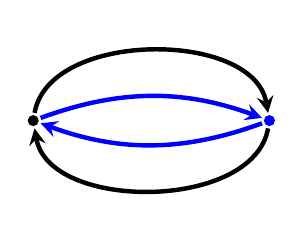
\begin{tikzpicture}
		\fill (0,0) circle (2pt);
		\fill[blue] (3,0) circle (2pt);
		\draw[ultra thick, -stealth,shorten <= 0.1cm, shorten >= 0.1cm] (0,0) to[bend left=80] (3,0);
		\draw[ultra thick, -stealth,shorten <= 0.1cm, shorten >= 0.1cm] (3,0) to[bend left=80] (0,0);
				\draw[ultra thick, -stealth,shorten <= 0.1cm, shorten >= 0.1cm, blue] (0,0) to[bend left=20] (3,0);
		\draw[ultra thick, -stealth,shorten <= 0.1cm, shorten >= 0.1cm, blue] (3,0) to[bend left=20] (0,0);
	\end{tikzpicture}
}
\hspace{1cm}
\subfloat[][ ]{%
	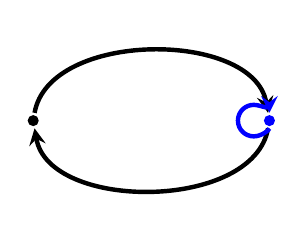
\begin{tikzpicture}
		\fill (0,0) circle (2pt);
\fill[blue] (3,0) circle (2pt);
\draw[ultra thick, -stealth,shorten <= 0.1cm, shorten >= 0.1cm] (0,0) to[bend left=80] (3,0);
\draw[ultra thick, -stealth,shorten <= 0.1cm, shorten >= 0.1cm] (3,0) to[bend left=80] (0,0);
\draw[ultra thick, -stealth,shorten <= 0.1cm, shorten >= 0.1cm, blue] (3,0) arc(0:-360:0.2);
	\end{tikzpicture}
}
\hspace{1cm}
\subfloat[][ ]{%
	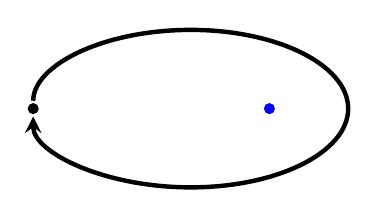
\begin{tikzpicture}
		\fill (0,0) circle (2pt);
		\fill[blue] (3,0) circle (2pt);
		\draw[ultra thick, -stealth,shorten <= 0.1cm, shorten >= 0.1cm] (0,0) arc(180:-180:2 and 1);
	\end{tikzpicture}
}
\caption{Double exchange of particles is topologically equivalent to one particle winding around the other. \textbf{(a)} Double exchange process of two particles. \textbf{(b)} Inner loop can be deformed in a continuous manner until it is infinitesimally small. \textbf{(c)} When the inner loop has been deformed to be of 0 size, the outer particle simply winds around the inner particle.}
\label{fig:doubleswap}
\end{figure}
\subsection{Statistics of the Excitations}
Why did we care so much about this model? The answer is in the interesting statistics exhibited. We are used to fermions and bosons. However, in two dimensions, there is a much richer zoo of possible excitation statistics.\note{Make interactive? Talk about deforming the loop. Go through the original proof!} 

Let us consider the double exchange process. In 3d, with fermions and bosons, this leads to the exact same wavefunction. Instead of computing it, we will compute what happens when one particle goes in a loop around the other, which is topologically equivalent (see Fig. \ref{fig:doubleswap}).

First, what happens when an e particle moves around an m particle? We see that this is mathematically identical to a Wilson loop (Fig. \ref{fig:wilsonloop}). This means that a double exchange procedure leads to a sign of -1! This is not possible in 3 dimensions, and is known as \emph{semionic} statistics.

Similarly, we can show due to commutativity that e and m particles are bosons.\note{Perhaps write it out?} Finally, we look at the e-m composite particle. This corresponds to a double exchange of an e particle with an m particle, as well as some e-m exchanges, leading to a sign of -1. Thus the composite particle is a fermion! This is the most basic example of \textbf{fractionalisation}.

\subsection{Outlook}
\begin{figure}
\subfloat[][ ]{%
	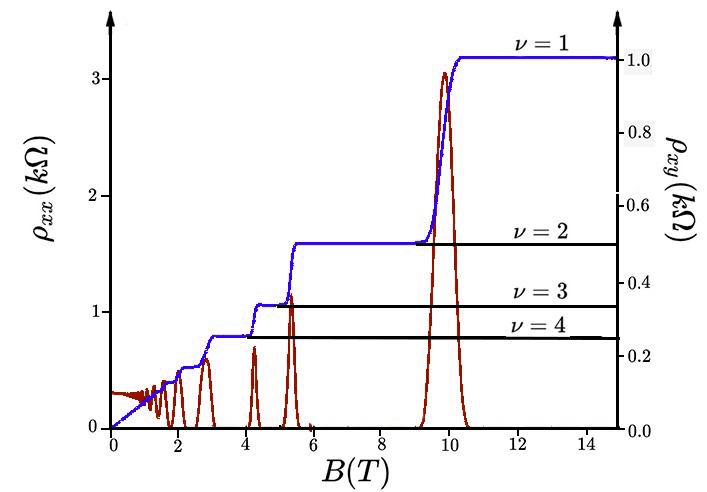
\includegraphics[height=5cm]{Rhoxy.jpg}
}
\hspace{1cm}
\subfloat[][ ]{%
	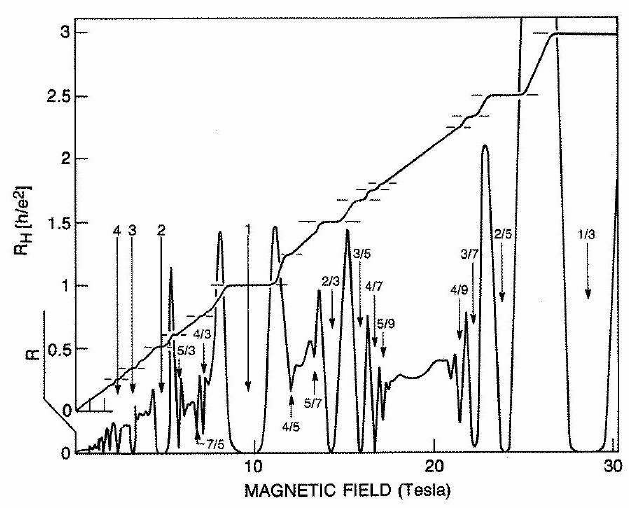
\includegraphics[height=5cm]{FQHE.png}
}
\caption{\textbf{(a)} Transverse resistivity in the integer Quantum hall effect shows peaks at integer Landau levels. Picture credit: wikimedia.org, Antikon, CC BY-SA 3.0. \textbf{(b)} A wide range of peaks are observed in the resistivity in the fractional Quantum Hall Effect. Picture from \cite{willett1987observation}.}
\label{fig:qhe}
\end{figure}
Can fractionalisation be observed in experiments? The answer is yes. The classic example is in the fractional Quantum Hall Effect (QHE). First, we must describe the integer QHE, which was discovered here in W\"{u}rzburg by von Klitzling. In the integer QHE, resistivities are observed at values
\[R_{xy} = \frac{h}{e^2\nu}\]
where $\nu$ takes on integer values. However, later, the fractional QHE was discovered (Fig. \ref{fig:qhe}(b)). These fractional resistivities could be explained by fractional charges, but the fundamental particle is always the electron, which has a charge of 1$e$. It turns out that the current is transported by fractional charges, leading to the fractionalised resistance.
\nocite{*}
%\bibliographystyle{ieeetr}
\bibliographystyle{apsrev4-2}
\bibliography{ref}
	\end{document}
